%%%%%%%%%%%%%%%%%%%%%%%%%%%%%%%%%%%%%%%%%%%%%%%%%%%%%%%%%%%%%%%%%%%%%%%%%%%%%%%%
%2345678901234567890123456789012345678901234567890123456789012345678901234567890
%        1         2         3         4         5         6         7         8

\documentclass[letterpaper, 10 pt, conference]{ieeeconf}  % Comment this line out if you need a4paper

%\documentclass[a4paper, 10pt, conference]{ieeeconf}      % Use this line for a4 paper

\IEEEoverridecommandlockouts                              % This command is only needed if 
                                                          % you want to use the \thanks command

\overrideIEEEmargins                                      % Needed to meet printer requirements.

%In case you encounter the following error:
%Error 1010 The PDF file may be corrupt (unable to open PDF file) OR
%Error 1000 An error occurred while parsing a contents stream. Unable to analyze the PDF file.
%This is a known problem with pdfLaTeX conversion filter. The file cannot be opened with acrobat reader
%Please use one of the alternatives below to circumvent this error by uncommenting one or the other
%\pdfobjcompresslevel=0
%\pdfminorversion=4

% See the \addtolength command later in the file to balance the column lengths
% on the last page of the document

% The following packages can be found on http:\\www.ctan.org
\usepackage{graphics} % for pdf, bitmapped graphics files
\usepackage{epsfig} % for postscript graphics files
%\usepackage{mathptmx} % assumes new font selection scheme installed
%\usepackage{times} % assumes new font selection scheme installed
\usepackage{amsmath} % assumes amsmath package installed
\usepackage{amssymb}  % assumes amsmath package installed
\usepackage{float}
\usepackage{xcolor}
\usepackage{pifont}
\usepackage{threeparttable}
\usepackage{mathtools}
\usepackage[ruled,vlined]{algorithm2e}
\newcommand\red[1]{\textcolor{red}{#1}}
\newcommand\blue[1]{\textcolor{blue}{#1}}

\usepackage{ulem} % for sout
\usepackage{kotex} % for korean
\usepackage{booktabs}
\usepackage{multirow}
\usepackage{tabularx}
\usepackage{graphicx} % for captions
\usepackage{subcaption}
\usepackage[font=footnotesize]{caption}
\usepackage{lipsum}
\captionsetup[figure]{justification=centering}
\captionsetup[subfigure]{justification=centering}

\usepackage{censor}
% \StopCensoring % Uncomment to show text
% \StartCensoring % Uncomment to hide text

% ---- Moderate but still subtle IEEE compression ----

% Equations
\setlength{\abovedisplayskip}{5pt plus 1pt minus 1pt}
\setlength{\belowdisplayskip}{5pt plus 1pt minus 1pt}
\setlength{\abovedisplayshortskip}{3pt plus 1pt minus 1pt}
\setlength{\belowdisplayshortskip}{3pt plus 1pt minus 1pt}

% Floats
\setlength{\textfloatsep}{7pt plus 1pt minus 2pt}
\setlength{\intextsep}{7pt plus 1pt minus 2pt}

% Bibliography (moderate tightening)
\usepackage{etoolbox}
\apptocmd{\thebibliography}{\setlength{\itemsep}{0pt}}{}{}
% ================================================================================

\title{\LARGE \bf
Contact-Aware Whole-Body Trajectory Optimization for Dual-Arm Aerial Box Transport with Slip-Aware Force Regulation
}


% \author{Albert Author$^{1}$ and Bernard D. Researcher$^{2}$% <-this % stops a space
% \thanks{*This work was not supported by any organization}% <-this % stops a space
% \thanks{$^{1}$Albert Author is with Faculty of Electrical Engineering, Mathematics and Computer Science,
%         University of Twente, 7500 AE Enschede, The Netherlands
%         {\tt\small albert.author@papercept.net}}%
% \thanks{$^{2}$Bernard D. Researcheris with the Department of Electrical Engineering, Wright State University,
%         Dayton, OH 45435, USA
%         {\tt\small b.d.researcher@ieee.org}}%
% }


\begin{document}



\maketitle
\thispagestyle{empty}
\pagestyle{empty}


%%%%%%%%%%%%%%%%%%%%%%%%%%%%%%%%%%%%%%%%%%%%%%%%%%%%%%%%%%%%%%%%%%%%%%%%%%%%%%%%
\begin{abstract}

Transporting bulky, box-shaped objects with an aerial robot is difficult for single-arm manipulators, since such objects cannot be enclosed by one gripper and must instead be held by friction between two opposing contacts. This couples the flying base, both arms, the contact forces, and the carried object, because the payload shifts the center of mass of the whole system and the squeezing force must be large enough to prevent slip during dynamic flight. This paper presents a contact-aware whole-body trajectory optimization framework for dual-arm aerial box transport. The entire pick-and-place task is formulated as a single optimal control problem that jointly plans the omnidirectional aerial base, both four-degree-of-freedom arms, and the object motion over the approach, grasp, transport, and release phases. Each end-effector is modeled as a deformable contact pad whose normal force is a smooth function of penetration, and a slip-aware constraint enforces a squeezing force sufficient for friction to hold the box against its expected acceleration, so the grip is firmed up exactly when it is needed. Collision avoidance is imposed on both the base and the carried object, so that the planner accounts for the full occupied volume of the robot--object system rather than the free-flight body alone. The framework is validated in simulation on an emergency-supply delivery scenario: the planner generates dynamically feasible trajectories that maintain a slip-free frictional grasp throughout acceleration and deceleration, and that carry the payload through a narrow awning-type window without collision.

\end{abstract}


%%%%%%%%%%%%%%%%%%%%%%%%%%%%%%%%%%%%%%%%%%%%%%%%%%%%%%%%%%%%%%%%%%%%%%%%%%%%%%%%
\section{Introduction}

\subsection{Background and Motivation}

Aerial manipulators have been widely studied as a means of extending robotic manipulation to elevated, remote, or cluttered environments where ground-based mobile manipulators have limited accessibility. In particular, omnidirectional aerial manipulators enlarge the controllable pose space of the flying base, allowing the robot to approach objects from diverse directions and to exploit a larger manipulation workspace than conventional underactuated multirotors.

Most existing aerial manipulation systems, however, rely on a single arm or a single end-effector. Although such systems are effective for simple grasping and interaction tasks, they are inherently limited when handling long, bulky, or box-shaped objects whose dimensions exceed the gripper aperture. A dual-arm aerial manipulator can overcome this limitation by contacting opposite sides of the object and holding it through frictional squeezing forces. This enables aerial transport of objects that cannot be enclosed by a single gripper.

At the same time, dual-arm aerial object transport introduces new planning challenges. Since the object is not rigidly attached to the robot, grasp stability depends on the contact locations, normal forces, friction coefficient, object weight, and object acceleration during transport. A fixed squeezing force may be insufficient during fast motion and may cause slip, while an excessive squeezing force can waste actuation authority and disturb the flying base. Moreover, once the object is grasped, the mass distribution and center of mass of the combined robot and object system change according to the arm configuration and the object pose. Therefore, the aerial base motion, both arm motions, contact forces, and object motion must be planned in a coupled manner.

%% 3-1. Overview of the proposed planning framework
\begin{figure}[!t] 
    \centering
    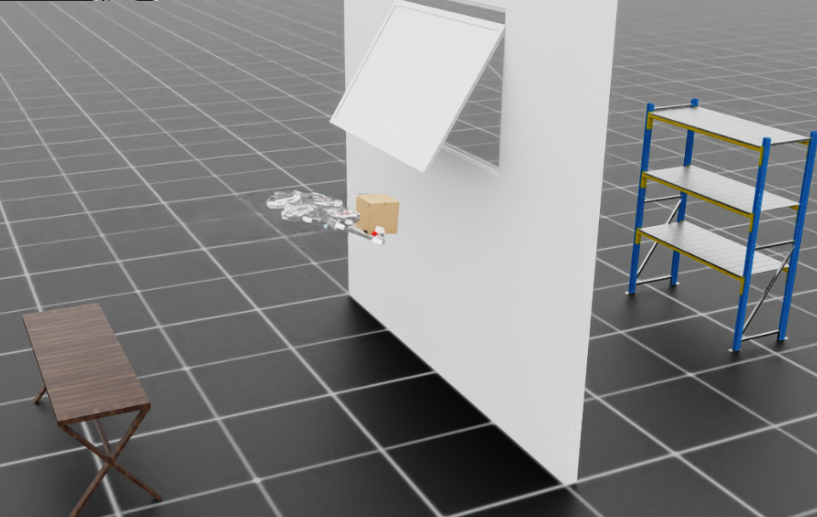
\includegraphics[width=0.9\linewidth]{images/thumbnail.png}
    \caption{Overview of the proposed whole-body trajectory planning for dual-arm aerial box transport through a narrow awning-type window. The planner generates a collision-free motion while considering the aerial base, both arms, and the carried object.}
    \label{fig:thumbnail}
\end{figure}

\subsection{Problem Description}

This paper addresses contact-aware whole-body trajectory optimization for dual-arm aerial pick-and-place. The target task consists of approaching a box, grasping it with two end-effectors, transporting it through the environment, and releasing it at a desired location. Each end-effector applies a normal squeezing force to one side of the box through a deformable contact pad, and the object is held by the friction generated at the two contact surfaces.

The main difficulty lies in generating a trajectory that is simultaneously feasible for the aerial base, both manipulators, the grasped object, and the contact interaction. Planning the flying base and the arms separately may produce motions that are kinematically plausible but dynamically unsuitable for stable aerial transport, especially because the payload changes the effective inertia and center of mass of the whole system. In addition, the optimizer must regulate the squeezing force according to the expected object motion so that sufficient friction is maintained during lift-off, acceleration, deceleration, and placement.

Collision avoidance must also account for the volume of the carried object. When the robot transports a box, the occupied space of the whole robot and object system changes significantly compared with the free-flight case. Therefore, the planner should consider not only the aerial base and the arms, but also the transported object when avoiding obstacles. In this work, this issue is handled by approximating the robot, object, and obstacles with ellipsoidal bodies and constructing obstacle clearance constraints from their Minkowski sums. This enables whole-body motion generation in cluttered environments, including a narrow-gate crossing scenario modeled as an awning-type window.

\subsection{Related Works}
% 2. Literature survey + research gap

Several recent studies have investigated whole-body planning and control for aerial manipulators. Lee et al. \cite{lee2025autonomous} proposed an omnidirectional aerial manipulator capable of hovering at arbitrary poses in $\mathrm{SE}(3)$, together with a geometric robust controller and a two-step trajectory-optimization-based whole-body motion planner. Their framework jointly considers the floating-base pose and the manipulator joint configuration, enabling grasping and pulling tasks near obstacles. Deng et al. \cite{deng2025whole} presented a whole-body integrated motion planning framework that simultaneously optimizes the trajectories of the quadrotor and the manipulator, and demonstrated various aerial manipulation skills such as grasping, lifting, pushing, and crossing through flexible waypoint constraints. These studies show the importance of coupled planning between the aerial base and the manipulator. However, they mainly focus on single-arm or single-end-effector systems, and therefore do not address coordinated dual-arm grasping, internal force regulation, or friction-based object holding for transporting bulky objects.

Collision-aware aerial manipulation in cluttered environments has also been explored. Yang et al. \cite{yang2025whole} proposed a whole-body motion planning and safety-critical control framework using superquadric geometric representations and proxy models to improve obstacle avoidance while considering dynamic feasibility. However, their main focus is on collision avoidance and safety-critical control of the aerial manipulator itself, rather than contact-rich manipulation of a carried object. In particular, previous works do not jointly optimize the aerial base, both arms, and the object motion while accounting for the volume of the transported object, nor do they regulate contact normal forces for stable frictional holding during dynamic dual-arm pick-and-place.
\par
To the best of our knowledge, no previous work simultaneously incorporates: (i) unified whole-body trajectory optimization for dual-arm aerial pick-and-place, (ii) contact-aware dual-arm aerial grasping through adjustable squeezing forces, and (iii) collision avoidance that accounts for the carried object during dynamic aerial transport.

\subsection{Contributions}
%% 3-2. main contributions
To summarize, the main contributions of this paper are as follows:
\begin{itemize}
    \item A unified whole-body trajectory optimization framework for dual-arm aerial pick-and-place, which formulates the entire task as a single optimal control problem. The proposed framework jointly optimizes the omnidirectional aerial base trajectory, the joint trajectories of both arms, and the object motion, instead of planning the flying base and manipulators separately.

    \item A contact-aware grasping model for friction-based dual-arm object holding using deformable end-effector pads. Each contact pad is modeled as a spring and damper element, allowing the normal squeezing force to be adjusted through pad deformation. This enables the optimizer to continuously increase or decrease the grasping force according to the expected object acceleration, maintaining a stable frictional grasp during fast transport without relying on rigid attachment or a single enveloping gripper.

    \item A collision avoidance formulation that accounts for the volume of the carried object during dynamic aerial transport. The robot, object, and obstacles are approximated using ellipsoids, and obstacle clearance constraints are constructed from their Minkowski sums. This allows the proposed method to generate feasible whole-body motions even when carrying a box through cluttered environments, as demonstrated in a narrow-gate crossing scenario modeled as an awning-type window.
\end{itemize}

\section{Controller design}
\label{sec:controller}

\subsection{System dynamics}
We select a coaxial tiltable quadrotor as the aerial base (Fig.~\ref{fig:modeling}), since its fully-actuated structure can generate large interaction forces required for aerial physical interaction (APhI); we refer to the resulting platform as an omnidirectional aerial manipulator (OAM). We consider the following system dynamics:
% 수식 1
\begin{equation}
\label{eq:system_dynamics}
\begin{aligned}
m\ddot{\boldsymbol{p}}
&=
{}^{\mathcal{W}}\!\boldsymbol{R}_{\mathcal{B}}\boldsymbol{f}
-
mg\boldsymbol{b}_3
+
\boldsymbol{d}_t
\\
\boldsymbol{J}_b \dot{\boldsymbol{\omega}}
&=
-
\boldsymbol{\omega}^{\wedge}
\boldsymbol{J}_b
\boldsymbol{\omega}
+
\boldsymbol{\tau}
+
\boldsymbol{d}_r
\end{aligned}
\end{equation}
where $\boldsymbol{p}$ and $\boldsymbol{\omega}$ are the base position and body angular velocity, ${}^{\mathcal{W}}\!\boldsymbol{R}_{\mathcal{B}}$ is the body-to-world rotation, and $\boldsymbol{d}_t,\boldsymbol{d}_r$ collect external disturbances. The net force $\boldsymbol{f}$ is the sum of four tilted rotor thrusts, with directions set by the tilt angles $(\alpha_i,\beta_i)$:
% 수식 2
\begin{equation}
\label{eq:total_force}
\begin{gathered}
\boldsymbol{f}
=
\sum_{i=1}^{4}
\boldsymbol{R}(\alpha_i)
\boldsymbol{R}(\beta_i)
T_i
\boldsymbol{e}_3
\\
\boldsymbol{R}(\alpha_i)
\boldsymbol{R}(\beta_i)
\boldsymbol{e}_3
=
\begin{bmatrix}
-s_{\beta_i}\\
s_{\alpha_i}c_{\beta_i}\\
c_{\alpha_i}c_{\beta_i}
\end{bmatrix}
\end{gathered}
\end{equation}
where $T_i$ is the thrust magnitude of rotor $i$ and $\boldsymbol{f}_i=\boldsymbol{R}(\alpha_i)\boldsymbol{R}(\beta_i)T_i\boldsymbol{e}_3$ denotes its thrust vector. The net torque combines each thrust moment arm $\boldsymbol{l}_i$ with the drag-induced reaction $\sigma_i k_f$:
% 수식 4
\begin{equation}
\label{eq:total_torque}
\begin{aligned}
\boldsymbol{\tau}
&=
\sum_{i=1}^{4}
\left[
\boldsymbol{l}_i \times \boldsymbol{f}_i
+
\sigma_i k_f \boldsymbol{f}_i
\right]
\end{aligned}
\end{equation}
where $\sigma_i=(-1)^{i+1}$ encodes the alternating rotor spin direction.

\subsection{Control allocation}

The OAM considered in this paper is illustrated in 

\begin{figure}[!t]
    \centering
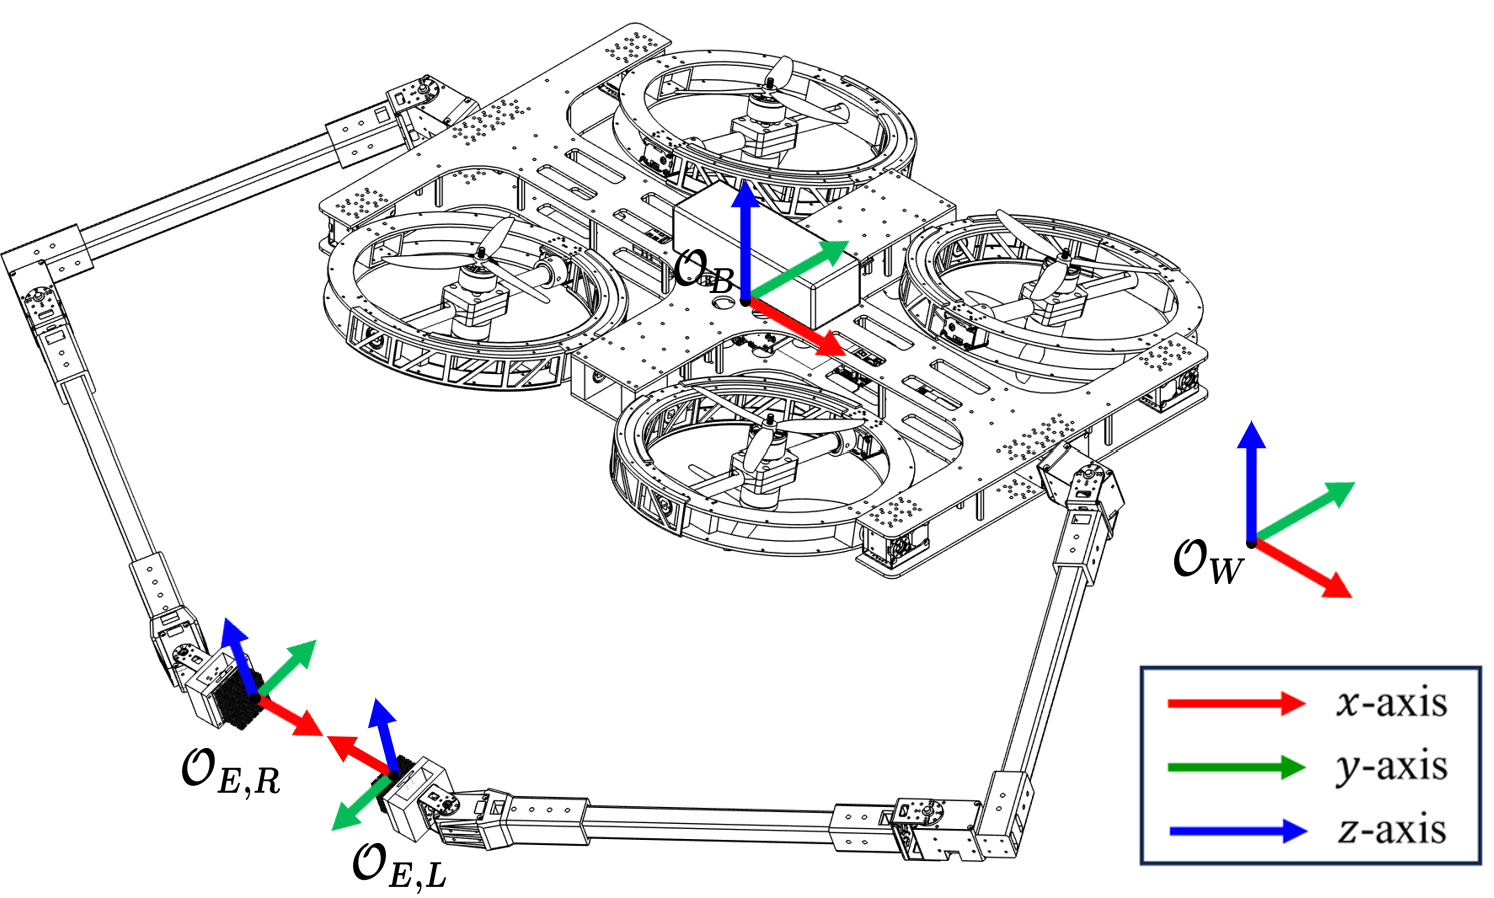
\includegraphics[width=0.9\linewidth]{images/modeling.png}
\vspace{-2mm}
    \caption{Three-dimensional models of the AM and Dual Arm, including their corresponding body frames.}
    \label{fig:modeling}
\end{figure}

% %수식 5
% \begin{equation}
% \label{eq:allocation_equation}
% \begin{aligned}
% \begin{bmatrix}
% \boldsymbol{f} \\
% \boldsymbol{\tau}
% \end{bmatrix}
% &=
% \boldsymbol{A}\boldsymbol{u},
% \qquad
% \boldsymbol{A}
% \in
% \mathbb{R}^{6 \times 12}
% \end{aligned}
% \end{equation}

% %수식6
% \begin{equation}
% \label{eq:control_input_uc}
% \begin{aligned}
% \boldsymbol{u}_c
% &=
% \begin{bmatrix}
% T_1 & \alpha_1 & \beta_1 & \cdots &
% T_4 & \alpha_4 & \beta_4
% \end{bmatrix}^{T}
% \end{aligned}
% \end{equation}


% %수식7
% \begin{equation}
% \label{eq:virtual_input_u}
% \begin{aligned}
% \boldsymbol{u}
% &=
% \begin{bmatrix}
% \boldsymbol{u}_1 \\
% \boldsymbol{u}_2 \\
% \boldsymbol{u}_3 \\
% \boldsymbol{u}_4
% \end{bmatrix},
% \qquad
% \boldsymbol{u}_i
% =
% \begin{bmatrix}
% -T_i \sin \beta_i \\
% T_i \sin \alpha_i \cos \beta_i \\
% T_i \cos \alpha_i \cos \beta_i
% \end{bmatrix},
% \qquad
% i = 1,\ldots,4.
% \end{aligned}
% \end{equation}

% %수식8
% \begin{equation}
% \label{eq:allocation_matrix_block}
% \begin{aligned}
% \boldsymbol{A}
% &=
% \begin{bmatrix}
% \boldsymbol{A}_1 &
% \boldsymbol{A}_2 &
% \boldsymbol{A}_3 &
% \boldsymbol{A}_4
% \end{bmatrix},
% \\
% \boldsymbol{A}_i
% &=
% \begin{bmatrix}
% 1 & 0 & 0 \\
% 0 & 1 & 0 \\
% 0 & 0 & 1 \\
% \sigma_i k_f & -l_{iz} & l_{iy} \\
% l_{iz} & \sigma_i k_f & -l_{ix} \\
% -l_{iy} & l_{ix} & \sigma_i k_f
% \end{bmatrix},
% \qquad
% \begin{aligned}
% i &= 1,\ldots,4, \\
% \sigma_i &= (-1)^{i+1}.
% \end{aligned}
% \end{aligned}
% \end{equation}


% 수식 압축버전
Stacking the per-rotor contributions, the net wrench is linear in the
per-rotor force vector $\boldsymbol{u}=[\boldsymbol{u}_1^\top \cdots \boldsymbol{u}_4^\top]^\top$,
with $\boldsymbol{u}_i=[-T_i s_{\beta_i},\, T_i s_{\alpha_i}c_{\beta_i},\, T_i c_{\alpha_i}c_{\beta_i}]^\top$:
\begin{equation}
\label{eq:allocation_equation}
\begin{bmatrix}\boldsymbol{f}\\ \boldsymbol{\tau}\end{bmatrix}
= \boldsymbol{A}\boldsymbol{u},\quad \boldsymbol{A}\in\mathbb{R}^{6\times12},\quad
\boldsymbol{A}_i=
\begin{bmatrix}
1&0&0\\ 0&1&0\\ 0&0&1\\
\sigma_i k_f & -l_{iz} & l_{iy}\\
l_{iz} & \sigma_i k_f & -l_{ix}\\
-l_{iy} & l_{ix} & \sigma_i k_f
\end{bmatrix},
\end{equation}
where $\boldsymbol{A}=[\boldsymbol{A}_1\,\cdots\,\boldsymbol{A}_4]$, $\sigma_i=(-1)^{i+1}$, and the actual
command $\boldsymbol{u}_c=[T_1,\alpha_1,\beta_1,\cdots,T_4,\alpha_4,\beta_4]^\top$ is recovered
by inverting~\eqref{eq:allocation_equation} following~\cite{lee2025autonomous}.

% grite사용 및 언급

\section{Whole-body motion planning}

This section overviews our whole-body trajectory generation
algorithm designed for an OAM.

\begin{table*}[!t]
\centering
\caption{Cost terms of the phase-dependent OCP objective.}
\label{tab:ocp_costs_tab}
\scriptsize
\renewcommand{\arraystretch}{1.05}
\begin{tabularx}{\textwidth}{@{}l l X l@{}}
\toprule
\textbf{Cost term} & \textbf{Expression} & \textbf{Role in the OCP} & \textbf{Active phase}\\
\midrule
\multicolumn{4}{@{}l}{\textit{(a) Grasp-force terms}}\\
$J_{\mathrm{grasp}}$    & $w_{\mathrm{grasp}}\!\left[(F_{L,k}-F_{d,k})^2+(F_{R,k}-F_{d,k})^2\right]$
  & Drives contact forces toward the desired grasp force $F_{d,k}$, keeping a firm friction grip. & Gr / Tr / Rel\\
$J_{\mathrm{internal}}$ & $w_{\mathrm{internal}}(F_{L,k}-F_{R,k})^2$
  & Balances the left/right force (internal-force regulation). & Gr / Tr\\
\addlinespace[1pt]
\multicolumn{4}{@{}l}{\textit{(b) Posture and alignment terms}}\\
$J_{\mathrm{open}}$  & $w_{\mathrm{open}}\textstyle\sum\nolimits_{s\in\{L,R\}}\sum\nolimits_{j=2}^{4}(\theta^{s}_{j,k}-\theta_{j,d})^2$
  & Holds the jaws open before contact so the pads straddle the object during descent. & App\\
$J_{\mathrm{align}}$ & $w_{\mathrm{align}}\!\left[(b_{x,k}-p_{x,k})^2+(b_{y,k}-p_{y,k})^2\right]$
  & Keeps the box under the base, minimizing CoM shift and disturbance torque. & All\\
$J_{\mathrm{tilt}}$  & $w_{\mathrm{tilt}}(q_{x,k}^2+q_{y,k}^2)$
  & Penalizes off-level roll/pitch tilt, $(q_{x,k},q_{y,k})$ the vector part of $q_k=\mathrm{quat}(\theta_k)$. & All\\
$J_{\mathrm{yaw}}$   & $w_{\mathrm{yaw}}\,\omega_{z,k}^2$
  & Suppresses gratuitous yaw motion (penalizes yaw rate, not value). & All\\
\addlinespace[1pt]
\multicolumn{4}{@{}l}{\textit{(c) Regularization and terminal terms}}\\
$J_{\mathrm{effort}}$ & $w_u\|u_k\|^2+w_v\|v_k\|^2$
  & Regularizes input/velocity for smooth, dynamically feasible motion. & All\\
$J_{N}$ & $w_{\mathrm{tilt}}(q_{x,N}^2+q_{y,N}^2)$
  & Terminal cost; keeps the final base attitude level at step $k=N$. & $k=N$\\
\bottomrule
\end{tabularx}
\\[1pt]
{\scriptsize\raggedright
$F_{d,k}=F_d$ during grasp/transport and $F_{d,k}=F_{\min}$ (relaxed) during release.
App/Gr/Tr/Rel $=$ approach/grasp/transport/release.\par}
\end{table*}

\begin{table*}[!t]
\centering
\caption{Constraints of the phase-dependent OCP.}
\label{tab:ocp_prob}
\scriptsize
\renewcommand{\arraystretch}{1.05}
\begin{tabularx}{\textwidth}{@{}c l X l@{}}
\toprule
\textbf{\#} & \textbf{Constraint} & \textbf{Expression} & \textbf{Holds for}\\
\midrule
C1  & Dynamics              & $v_{k+1}=v_k+u_k\Delta t,\quad q_{k+1}=q_k+v_{k+1}\Delta t$ & all $k$\\
C2  & Object support        & $b_k=\mathrm{pick}\ (\mathrm{App,Gr}),\quad b_k=\mathrm{place}\ (\mathrm{Rel})$ & App, Gr, Rel\\
C3  & No-slip carry         & $b_k=p_k+R(\theta_k)\,m^{b}_k$ & grip\\
C4  & Grip geometry         & $p^{b}_{L,y,k}=p^{b}_{R,y,k},\quad p^{b}_{L,z,k}=p^{b}_{R,z,k}$ & grip\\
C5  & Slip-aware force      & $F_{L,k}\ge F^{\mathrm{set}}_k,\quad F_{R,k}\ge F^{\mathrm{set}}_k$ & Tr\\
C6  & Collision keep-out    & $g_{\mathrm{obs}}(b_k)\ge 0,\quad g_{\mathrm{obs}}(p_k)\ge 0$ & Tr\\
C7  & Clearance \& corridor & $g_{\mathrm{clr}}(p_k)\ge 0,\ \ g_{\mathrm{ee}}(p^{w}_{i,k})\ge0\ (i{\in}\{L,R\}),\ \ g_{\mathrm{cyl}}(b_k)\ge 0$ & all $k$\\
C8  & Descent centering     & $\tfrac12\big(p^{w}_{L,xy,k}+p^{w}_{R,xy,k}\big)=b_{xy,k}$ & App (descent)\\
C9  & Arm mirror            & $\theta^{L}_{1,k}+\theta^{R}_{1,k}=0,\quad \theta^{L}_{j,k}=\theta^{R}_{j,k}\ (j{=}2,3,4)$ & all $k$\\
C10 & Parallel jaw          & $\theta^{s}_{2,k}-\theta^{s}_{3,k}-\theta^{s}_{4,k}=0,\quad s\in\{L,R\}$ & all $k$\\
C11 & Bounds                & $\underline{\psi}\le\psi_k\le\overline{\psi},\ \ \|v_k\|_\infty\le v_{\max},\ \ \|u_k\|_\infty\le u_{\max}$ & all $k$\\
C12 & Boundary conditions   & $q_0=(p_{\mathrm{home}},0,\psi_{\mathrm{start}}),\ \ v_0=0,\ \ b_N=\mathrm{place}$ & endpoints\\
\bottomrule
\end{tabularx}
\\[1pt]
{\scriptsize\raggedright
grip $=\mathrm{Gr}\cup\mathrm{Tr}\cup\mathrm{Rel}$;\ $m^{b}_k$ is the pad midpoint in the base frame.\par}
\end{table*}

\subsection{Offline trajectory generation}

We generate the whole-body reference trajectory offline by solving a single optimal control problem (OCP) that couples the aerial base, both arms, the carried object, and the contact forces over the entire pick-and-place task. The task is transcribed by direct transcription into $N$ uniform intervals of length $\Delta t$, and the decision variables at each knot $k$ are the configuration $q_k$, its velocity $v_k$, the acceleration input $u_k$, and the object position $b_k$. The configuration $q_k\in\mathbb{R}^{14}$ stacks the floating-base position, the base attitude, and the eight arm joints. The base attitude is represented in exponential coordinates by a rotation vector, so that the whole configuration evolves in a Euclidean space and the integration can be written as a simple double integrator (C1). Rather than planning the base and the arms separately, this single problem optimizes them jointly together with the object and the squeezing forces, which is essential because the payload changes the effective inertia and center of mass of the whole system.

For planning purposes the fully-actuated base is modeled at the acceleration level as a double integrator driven by $u_k$, while the base and arm velocities and accelerations are constrained to admissible ranges (C11). This decouples the offline geometry-and-force planning from the low-level allocation and control of Section~\ref{sec:controller}: the OAM realizes the commanded accelerations through the wrench allocation~\eqref{eq:allocation_equation}, and the geometric controller tracks the resulting reference. The reference therefore needs only to be kinematically smooth, dynamically consistent at the rigid-body level, and contact-feasible.

The task is divided into four phases---approach, grasp, transport, and release---scheduled over fixed per-phase durations. The phases share identical dynamics and a single smooth contact model, and differ only in which cost terms and constraints are active, forming a time-indexed finite-state machine over the horizon. During approach and grasp the object rests on the pick-up support, during release it sits at the placement, and these supporting positions are imposed as the object-support constraint (C2). The boundary conditions (C12) fix the home pose, zero initial velocity, and the final object placement, and the optimizer discovers the intermediate flight, grasp, and carry that connect them.

The grasp is modeled through deformable end-effector pads rather than a rigid attachment. Each pad is treated as a spring--damper element, so the normal contact force is a smooth $C^1$ function of a virtual penetration depth between the pad and the object face, and the left/right forces $F_{L,k},F_{R,k}$ are derived quantities of the configuration rather than independent decision variables. This avoids any complementarity or active-set switching and keeps the OCP smooth and differentiable for a gradient-based solver. While the object is held, the no-slip carry constraint (C3) ties the object to the end-effector pad midpoint, and the grip-geometry constraints (C4, C8--C10) keep the two pads symmetric, parallel-jawed, and centered on the object face, so that closing the grip is a pure squeeze along the contact normal.

The squeezing force is regulated according to the expected object motion so that friction alone can hold the object during dynamic transport. From the object free body, the per-contact normal force needed to carry the box at an upward acceleration $a_z$ is $F^{\mathrm{set}}=m_o(g+a_z)/(2\mu)$, where $\mu$ is the contact friction coefficient. This slip-aware setpoint is computed along the planned transport profile and imposed as a hard lower bound on both contact forces (C5), so the optimizer raises the squeeze during the acceleration and deceleration phases and may relax it otherwise. Embedding the no-slip limit directly as a constraint, rather than tracking a fixed force, lets the planner spend just enough internal force to prevent slip throughout the carry. The grasp-force cost $J_{\mathrm{grasp}}$ then pulls the contact forces toward the desired level $F_{d,k}$, while $J_{\mathrm{internal}}$ balances the left and right forces to regulate the internal squeezing force.

Collision avoidance accounts for the volume of the carried object during transport. The clearance constraints (C6, C7) are imposed on both the base and the object, so that the planner reasons about the full occupied space of the robot--object system rather than the free-flight body alone; the corridor and window terms confine the object as it threads the narrow awning-type opening. Because the object-support and clearance constraints couple the object to the base and arms through the no-slip carry, a trajectory that respects the object's volume is generated jointly with the base and arm motion. To shape the whole-body motion, the alignment cost $J_{\mathrm{align}}$ keeps the object beneath the base to minimize the center-of-mass shift and the resulting disturbance torque, $J_{\mathrm{tilt}}$ and $J_{\mathrm{yaw}}$ keep the base attitude near level, $J_{\mathrm{open}}$ holds the jaws open before contact, and $J_{\mathrm{effort}}$ together with the terminal cost $J_N$ regularize the inputs for a smooth, level final pose. The complete objective and constraints are summarized in Tables~\ref{tab:ocp_costs_tab} and~\ref{tab:ocp_prob}.

The resulting OCP is

\begin{equation}
\label{eq:ocp_problem}
\begin{aligned}
\min_{\{q_k,\,v_k,\,u_k,\,b_k\}}\ & \sum_{k=0}^{N-1} J_k + J_N\\[2pt]
\text{s.t.}\ & (\mathrm{C1})\text{--}(\mathrm{C12}),\quad \forall k,\\[3pt]
J_k =\ & J_{\mathrm{grasp}}+J_{\mathrm{internal}}+J_{\mathrm{open}}+J_{\mathrm{align}}\\
  & +J_{\mathrm{tilt}}+J_{\mathrm{yaw}}+J_{\mathrm{effort}},
\end{aligned}
\end{equation}

where each cost term is active only in its corresponding phase,
and $J_N$ is a terminal cost. The cost terms and
constraints~(C1)--(C12) are detailed in
Tables~\ref{tab:ocp_costs_tab}--\ref{tab:ocp_prob}.

\section{Experimental results}

\subsection{Experimental Setup}
The proposed framework is evaluated on an emergency-supply delivery scenario, in which the robot retrieves a payload outside a building, passes through a partially opened awning-type window, and places it at a predefined location inside.
The transported box represents a surrogate payload for emergency items such as a compact fire extinguisher, a first-aid kit, or medical supplies.
Two experiments are conducted under this scenario: a dual-arm pick-and-place task that examines stable payload transport, and a narrow-gate crossing task that examines whole-body trajectory generation through the constrained opening while carrying the payload.

The platform is the coaxial tiltable quadrotor of Section~\ref{sec:controller}, equipped with two symmetric four-degree-of-freedom arms terminating in deformable contact pads. The offline OCP~\eqref{eq:ocp_problem} is transcribed and solved with CasADi and the interior-point solver IPOPT, warm-started from a dynamically consistent kinematic guess. The resulting reference is replayed in the Isaac Sim / Isaac Lab physics engine (PhysX) at $200\,\mathrm{Hz}$, where the base is driven by the geometric SE(3) tracking controller and the box is held only by the friction of the two squeezing pads, so that an insufficient grip manifests as physical slip. The main system, contact, and OCP parameters are listed in Table~\ref{tab:params}.

The OCP horizon spans $N=108$ intervals at $\Delta t = 0.1\,\mathrm{s}$, giving a $10.8\,\mathrm{s}$ trajectory split into the four phases with durations $(3.0,\,1.6,\,5.0,\,1.2)\,\mathrm{s}$ for approach, grasp, transport, and release. The same robot, box, contact, and weighting parameters are used in both experiments; only the environment (free transport vs.\ the awning window) differs.

\begin{table}[!t]
\centering
\caption{System, contact, and OCP parameters.}
\label{tab:params}
\footnotesize
\renewcommand{\arraystretch}{1.1}
\begin{tabular}{@{}llc@{}}
\toprule
\textbf{Group} & \textbf{Parameter} & \textbf{Value}\\
\midrule
\multirow{2}{*}{Robot}
 & base inertia $\boldsymbol{J}_b$ [kg\,m$^2$] & $\mathrm{diag}(0.082,0.156,0.234)$\\
 & arms ($\times2$), DoF per arm & $2,\ 4$\\
\addlinespace[1pt]
\multirow{2}{*}{Payload}
 & box size [m] & $0.26\times0.26\times0.262$\\
 & box mass $m_o$ [kg] & $0.4$\\
\addlinespace[1pt]
\multirow{3}{*}{Contact}
 & friction coefficient $\mu$ & $0.7$\\
 & pad stiffness $k$ [N/m] & $2000$\\
 & number of contacts $n$ & $2$\\
\addlinespace[1pt]
\multirow{3}{*}{OCP}
 & horizon $N$, step $\Delta t$ [s] & $108,\ 0.1$\\
 & phase durations [s] & $3.0/1.6/5.0/1.2$\\
 & grasp squeeze $F_d$ [N] & $60$\\
\bottomrule
\end{tabular}
\end{table}


\subsection{Dual-Arm Pick-and-Place}
The first experiment considers a last-mile logistics delivery task, in which the robot grasps a payload, transports it, and releases it at the destination, as performed by autonomous delivery drones.
The objective is to verify that the slip-aware force regulation sustains a stable frictional grasp throughout the acceleration and deceleration phases of transport.

The robot starts from a home hover above the pick-up site. The box initially rests on a desk and must be relocated onto the top shelf of a storage rack about $4\,\mathrm{m}$ away laterally and roughly $1.1\,\mathrm{m}$ higher. The planner produces the full approach--grasp--transport--release sequence: the open jaws descend vertically and straddle the box, the squeeze is built up at rest, the box is lifted and carried up and over to the shelf, and the grip is relaxed at placement.

The slip-aware behavior is the key result of this experiment. As the box is lifted and accelerated, the slip-aware setpoint $F^{\mathrm{set}}_k$, computed from the commanded vertical acceleration along the transport profile, rises from its floor of $2\,\mathrm{N}$ to about $11.8\,\mathrm{N}$ at the peak acceleration. The optimizer keeps both contact forces above this lower bound at all times (mean transport squeeze $\approx 19\,\mathrm{N}$, peak $22\,\mathrm{N}$), so the available friction always exceeds the inertial load on the payload. In the Isaac Sim replay the box is carried with no observable slip between the pads and the box throughout the full acceleration and deceleration profile, and the base tracks the planned reference with a position RMSE of about $0.05\,\mathrm{m}$ while staying near level. This confirms that scaling the squeeze with the expected acceleration, rather than applying a fixed force, is sufficient to prevent slip during dynamic transport.

\subsection{Narrow-Gate Crossing}
The second experiment considers the full delivery scenario, in which the grasped payload is carried through the partially opened awning-type window without collision.
The objective is to verify that the object-aware collision avoidance produces a feasible whole-body trajectory while the slip-aware grasp is maintained throughout the constrained passage.

The awning-type window is modeled as a thin wall whose opening spans about $1.7\,\mathrm{m}$ laterally and roughly $1\,\mathrm{m}$ vertically beneath the slanted awning, with a small clearance margin of $0.04\,\mathrm{m}$ enforced between the window frame and any part of the robot--object system. Because the opening sits above the carry height, the box cannot simply be pushed straight through: the robot must lift the forward-carried box up to the opening and thread it through while keeping the base clear of the frame.

The object-aware collision avoidance is decisive here. The keep-out and clearance constraints are imposed on both the box and the base, so the planner reasons about the full occupied volume of the robot--object system rather than the free-flight body alone. As a result, the optimizer discovers a whole-body motion in which the base pitches nose-up to raise the box into the elevated opening and holds that tilt while crossing, so that the box passes through the lateral and vertical limits of the window while the body simultaneously clears the frame at the prescribed margin. Throughout this constrained passage the slip-aware lower bound remains active and the friction grasp is maintained, so the box is carried through the window without slipping. A trajectory that ignored the carried object would have driven the box into the frame at the same clearance margin, whereas the proposed formulation yields a collision-free passage.

\subsection{Results and Discussion}
% ------------------<내용>----------------------------
% 두 실험 수치 종합. slip 거리, 추적 RMSE, CoM shift, clearance/통과 성공 여부, 계산 시간 등 정리.
% 한계 먼저 깔기: baseline 비교랑 ablation 안 함 + 시뮬만 함 → future work에서 비교실험/실기 실험 언급해서 reviewer 방어.


First, the slip-aware force regulation maintained a stable frictional grasp throughout transport.
During the acceleration and deceleration phases, the desired grasp force $F_{d,k}$ increased in response to the larger inertial load on the payload, and the resulting normal forces kept the relative slip at the contact pads at zero.
This confirms that adjusting the squeezing force according to the expected object acceleration, rather than applying a fixed force, is sufficient to prevent slip during dynamic motion.

Second, the object-aware collision avoidance enabled the robot to cross the narrow awning-type window while carrying the box.
Because the obstacle clearance constraints are constructed from the Minkowski sums of the ellipsoidal robot, object, and obstacles, the planner accounts for the full occupied volume of the robot--object system rather than the free-flight body alone.
A trajectory that neglects the carried object would have placed the box in collision with the window frame at the same clearance margin, whereas the proposed formulation generated a collision-free passage.

Third, formulating the entire task as a single optimal control problem allowed the aerial base, both arms, and the object motion to be coordinated within one trajectory.
Since the payload shifts the effective center of mass of the combined system, planning the base and the arms separately would induce a disturbance torque, while the unified formulation compensated for the CoM shift through the alignment cost $J_{\mathrm{align}}$ and kept the base attitude near level during transport.

These results are obtained in simulation, and the present study does not include a quantitative comparison against baseline planners or an ablation of the individual cost terms.
Future work will therefore extend the evaluation with comparisons against decoupled base--arm planning and fixed-force grasping, and with real-world experiments on the physical platform.
\section{CONCLUSIONS}

This paper presented a contact-aware whole-body trajectory optimization framework for dual-arm aerial box transport.
The entire pick-and-place task is formulated as a single optimal control problem that jointly plans the omnidirectional aerial base, both arms, and the object motion.
A deformable-pad contact model regulates the squeezing force according to the expected object acceleration, and an ellipsoidal Minkowski-sum formulation accounts for the volume of the carried object during collision avoidance.
In simulation, the planner generated dynamically feasible trajectories that maintained a slip-free grasp throughout transport and crossed a narrow awning-type window while carrying the payload.
Future work will extend the evaluation with comparisons against decoupled base--arm planning and fixed-force grasping, and validate the framework through real-world experiments on the physical platform.

 

\addtolength{\textheight}{-12cm}   % This command serves to balance the column lengths
                                  % on the last page of the document manually. It shortens
                                  % the textheight of the last page by a suitable amount.
                                  % This command does not take effect until the next page
                                  % so it should come on the page before the last. Make
                                  % sure that you do not shorten the textheight too much.

%%%%%%%%%%%%%%%%%%%%%%%%%%%%%%%%%%%%%%%%%%%%%%%%%%%%%%%%%%%%%%%%%%%%%%%%%%%%%%%%



%%%%%%%%%%%%%%%%%%%%%%%%%%%%%%%%%%%%%%%%%%%%%%%%%%%%%%%%%%%%%%%%%%%%%%%%%%%%%%%%



%%%%%%%%%%%%%%%%%%%%%%%%%%%%%%%%%%%%%%%%%%%%%%%%%%%%%%%%%%%%%%%%%%%%%%%%%%%%%%%%
\section*{APPENDIX}

Appendixes should appear before the acknowledgment.

\section*{ACKNOWLEDGMENT}

The preferred spelling of the word ÒacknowledgmentÓ in America is without an ÒeÓ after the ÒgÓ. Avoid the stilted expression, ÒOne of us 


%%% REFERENCE
\bibliographystyle{IEEEtran}
\bibliography{bibtex/refer}
\vfill





\end{document}
